\chapter{Planejamento das Atividades}\label{plan}

Este cap\'itulo apresenta as atividades a serem realizadas para a elabora\c{c}\~ao desta tese.
As seguintes atividades j\'a foram realizadas:

\begin{enumerate}
	\item Defini\c{c}\~ao formal de um sistema de tipos para Haskell que d\^e suporte a classes de tipos com 
	      m\'ultiplos par\^ametros sem a necessidade de extens\~oes.
	\item Implementa\c{c}\~ao de um \emph{front-end} para Haskell que utilize o sistema de tipos proposto.	 
\end{enumerate}

As seguintes atividades devem ser realizadas para alcan\c{c}ar os objetivos tra\c{c}ados nesta tese:

\begin{enumerate}
	\item Modifica\c{c}\~ao do sistema de tipos j\'a elaborado para permitir a defini\c{c}\~ao opcional de
	      classes de tipos. Para isso, deve-se modificar o sistema de tipos para acomodar a utiliza\c{c}\~ao
	      de opera\c{c}\~oes de supremo, definidas na se\c{c}\~ao \ref{lcg}.
	\item Modifica\c{c}\~ao do prot\'otipo para permitir a defini\c{c}\~ao opcional de classes de tipos.
	\item Avalia\c{c}\~ao do prot\'otipo para infer\^encia de tipos de bibliotecas Haskell que utilizam depend\^encias
	      funcionais ou fam\'ilias de tipos. 
	\item Elabora\c{c}\~ao de restri\c{c}\~oes sobre defini\c{c}\~oes de classes e inst\^ancias para garantir a 
	      termina\c{c}\~ao do algoritmo para satisfazibilidade de restri\c{c}\~oes.
	\item Prova de corretude do algoritmo de infer\^encia de tipos com rela\c{c}\~ao ao sistema de tipos
	      proposto.
	\item Prova que o sistema de tipos proposto possui as propriedades de tipo e tipagem principal.
\end{enumerate}

At\'e o presente momento o seguinte artigo foi publicado:
\begin{itemize}
	\item \emph{A Solution to Haskell's Multi-Parameter Type Class Dilemma}. Este artigo apresenta o sistema de tipos
	      descrito no cap\'itulo \ref{capmptc} deste trabalho. Publicado no XIII Simp\'osio Brasileiro
	      de Linguagens de Programa\c{c}\~ao em 2009.
\end{itemize}

Os seguintes artigos ainda ser\~ao elaborados com os resultados futuros deste trabalho:
\begin{itemize}
	\item \emph{Optional and Multi-Parameter Type Classes for Haskell}. Apresenta\c{c}\~ao da vers\~ao final do sistema de
	      tipos e algoritmo de infer\^encia proposto neste trabalho.
	\item \emph{Haskell and Principal Typings}. Trabalho que descrever\'a a prova formal da propriedade de tipagem
	      principal para o sistema de tipos proposto.
\end{itemize}

A figura \ref{sumario} apresenta o sum\'ario proposto para esta tese. As se\c{c}\~oes a serem elaboradas est\~ao em 
destaque.

\begin{figure}[htp]			
	\centering
	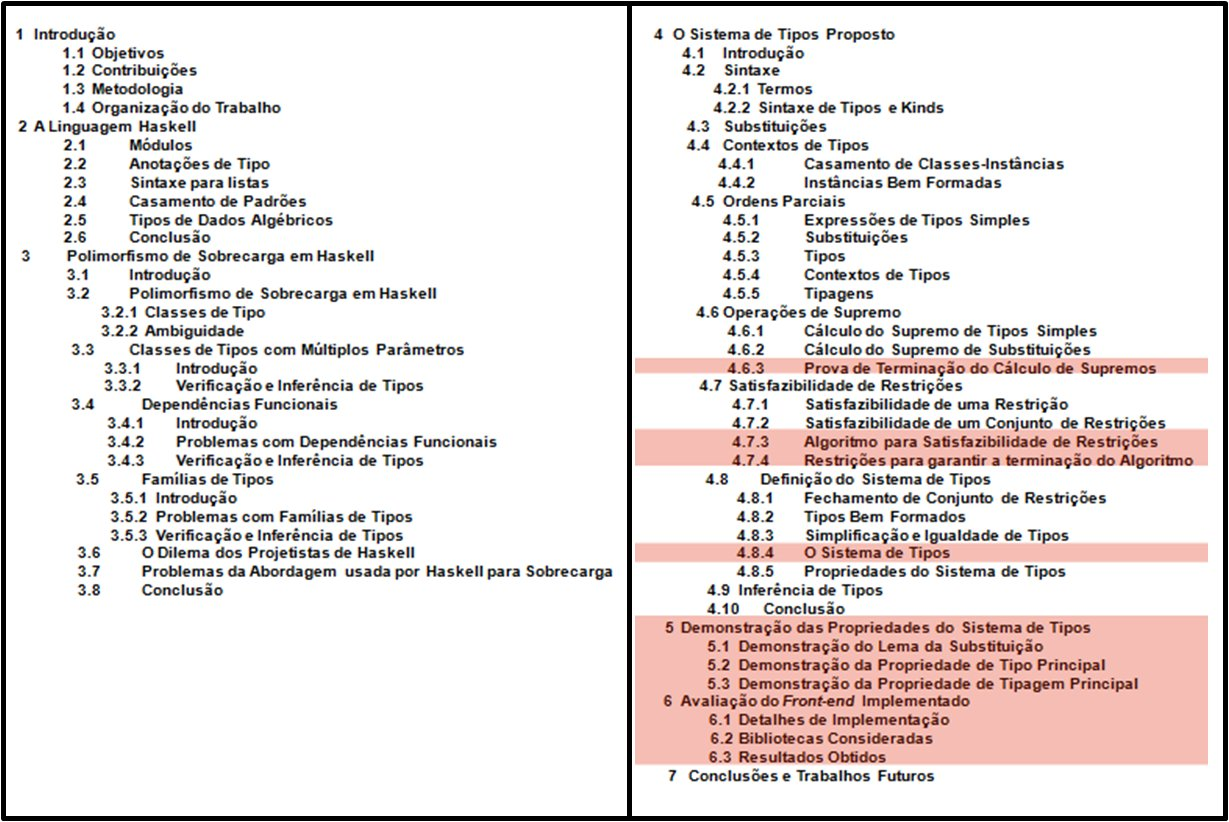
\includegraphics[scale=0.5]{sumario.jpg}
	\caption{Sum\'ario da Tese}
	\label{sumario}
\end{figure}		

O cronograma das atividades a serem realizadas \'e apresentado na figura \ref{cronograma}.

\begin{figure}[t]			
	\centering
	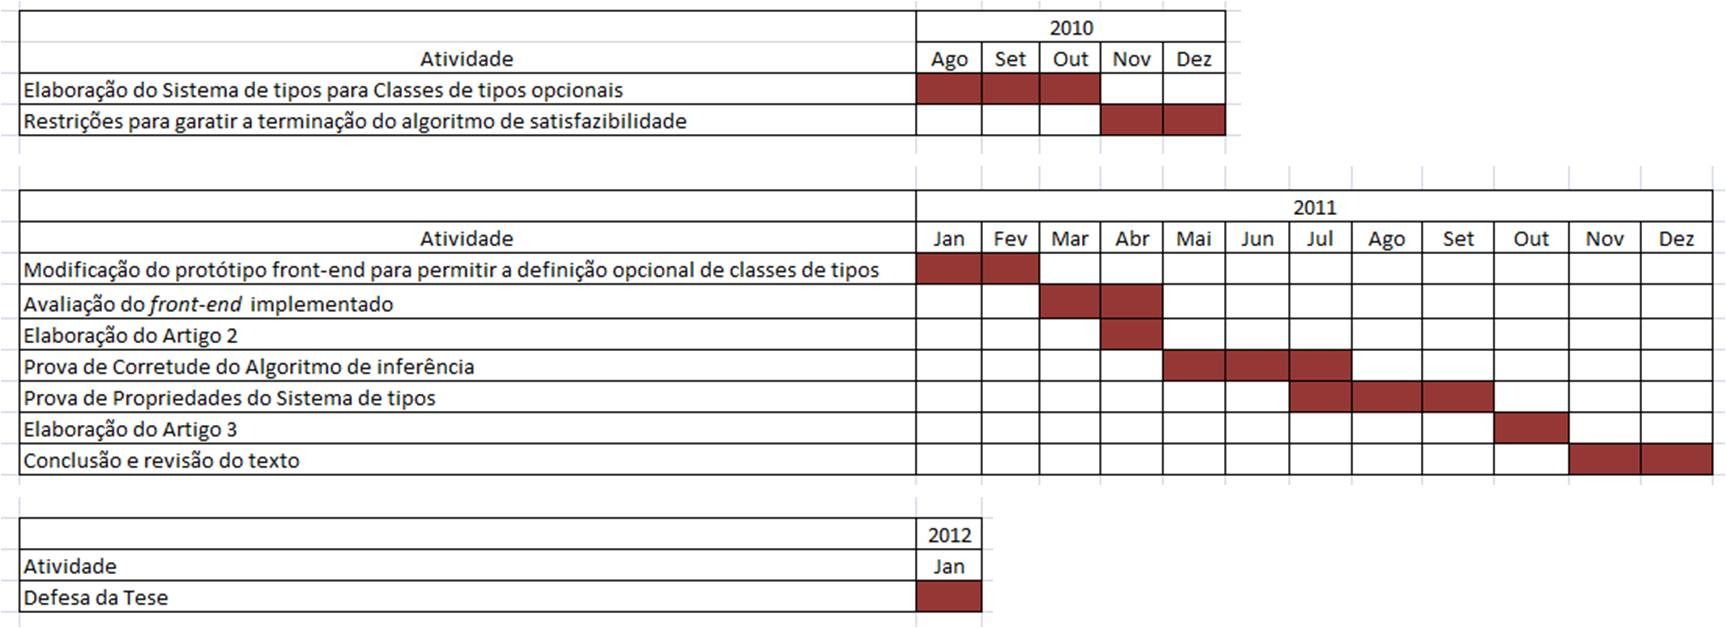
\includegraphics[scale=0.5]{cronograma.jpg}
	\caption{Cronograma das Atividades}
	\label{cronograma}
\end{figure}	
